\documentclass{ximera}

\title{Practice for Eigenvalue Method with Complex Roots}

%\auor{Matthew Charnley and Jason Nowell}
\usepackage[margin=1.5cm]{geometry}
\usepackage{indentfirst}
\usepackage{sagetex}
\usepackage{lipsum}
\usepackage{amsmath}
\usepackage{mathrsfs}


%%% Random packages added without verifying what they are really doing - just to get initial compile to work.
\usepackage{tcolorbox}
\usepackage{hypcap}
\usepackage{booktabs}%% To get \toprule,\midrule,\bottomrule etc.
\usepackage{nicefrac}
\usepackage{caption}
\usepackage{units}

% This is my modified wrapfig that doesn't use intextsep
\usepackage{mywrapfig}
\usepackage{import}



%%% End to random added packages.


\graphicspath{
    {./figures/}
    {./../figures/}
    {./../../figures/}
}
\renewcommand{\log}{\ln}%%%%
\DeclareMathOperator{\arcsec}{arcsec}
%% New commands


%%%%%%%%%%%%%%%%%%%%
% New Conditionals %
%%%%%%%%%%%%%%%%%%%%


% referencing
\makeatletter
    \DeclareRobustCommand{\myvref}[2]{%
      \leavevmode%
      \begingroup
        \let\T@pageref\@pagerefstar
        \hyperref[{#2}]{%
	  #1~\ref*{#2}%
        }%
        \vpageref[\unskip]{#2}%
      \endgroup
    }%

    \DeclareRobustCommand{\myref}[2]{%
      \leavevmode%
      \begingroup
        \let\T@pageref\@pagerefstar
        \hyperref[{#2}]{%
	  #1~\ref*{#2}%
        }%
      \endgroup
    }%
\makeatother

\newcommand{\figurevref}[1]{\myvref{Figure}{#1}}
\newcommand{\figureref}[1]{\myref{Figure}{#1}}
\newcommand{\tablevref}[1]{\myvref{Table}{#1}}
\newcommand{\tableref}[1]{\myref{Table}{#1}}
\newcommand{\chapterref}[1]{\myref{chapter}{#1}}
\newcommand{\Chapterref}[1]{\myref{Chapter}{#1}}
\newcommand{\appendixref}[1]{\myref{appendix}{#1}}
\newcommand{\Appendixref}[1]{\myref{Appendix}{#1}}
\newcommand{\sectionref}[1]{\myref{\S}{#1}}
\newcommand{\subsectionref}[1]{\myref{subsection}{#1}}
\newcommand{\subsectionvref}[1]{\myvref{subsection}{#1}}
\newcommand{\exercisevref}[1]{\myvref{Exercise}{#1}}
\newcommand{\exerciseref}[1]{\myref{Exercise}{#1}}
\newcommand{\examplevref}[1]{\myvref{Example}{#1}}
\newcommand{\exampleref}[1]{\myref{Example}{#1}}
\newcommand{\thmvref}[1]{\myvref{Theorem}{#1}}
\newcommand{\thmref}[1]{\myref{Theorem}{#1}}


\renewcommand{\exampleref}[1]{ {\color{red} \bfseries Normally a reference to a previous example goes here.}}
\renewcommand{\figurevref}[1]{ {\color{red} \bfseries Normally a reference to a previous figure goes here.}}
\renewcommand{\tablevref}[1]{ {\color{red} \bfseries Normally a reference to a previous table goes here.}}
\renewcommand{\Appendixref}[1]{ {\color{red} \bfseries Normally a reference to an Appendix goes here.}}
\renewcommand{\exercisevref}[1]{ {\color{red} \bfseries Normally a reference to a previous exercise goes here.}}



\newcommand{\R}{\mathbb{R}}

%% Example Solution Env.
\def\beginSolclaim{\par\addvspace{\medskipamount}\noindent\hbox{\bf Solution:}\hspace{0.5em}\ignorespaces}
\def\endSolclaim{\par\addvspace{-1em}\hfill\rule{1em}{0.4pt}\hspace{-0.4pt}\rule{0.4pt}{1em}\par\addvspace{\medskipamount}}
\newenvironment{exampleSol}[1][]{\beginSolclaim}{\endSolclaim}

%% General figure formating from original book.
\newcommand{\mybeginframe}{%
\begin{tcolorbox}[colback=white,colframe=lightgray,left=5pt,right=5pt]%
}
\newcommand{\myendframe}{%
\end{tcolorbox}%
}

%%% Eventually return and fix this to make matlab code work correctly.
%% Define the matlab environment as another code environment
%\newenvironment{matlab}
%{% Begin Environment Code
%{ \centering \bfseries Matlab Code }
%\begin{code}
%}% End of Begin Environment Code
%{% Start of End Environment Code
%\end{code}
%}% End of End Environment Code


% this one should have a caption, first argument is the size
\newenvironment{mywrapfig}[2][]{
 \wrapfigure[#1]{r}{#2}
 \mybeginframe
 \centering
}{%
 \myendframe
 \endwrapfigure
}

% this one has no caption, first argument is size,
% the second argument is a larger size used for HTML (ignored by latex)
\newenvironment{mywrapfigsimp}[3][]{%
 \wrapfigure[#1]{r}{#2}%
 \centering%
}{%
 \endwrapfigure%
}
\newenvironment{myfig}
    {%
    \begin{figure}[h!t]
        \mybeginframe%
        \centering%
    }
    {%
        \myendframe
    \end{figure}%
    }


% graphics include
\newcommand{\diffyincludegraphics}[3]{\includegraphics[#1]{#3}}
\newcommand{\myincludegraphics}[3]{\includegraphics[#1]{#3}}
\newcommand{\inputpdft}[1]{\subimport*{../figures/}{#1.pdf_t}}


%% Not sure what these even do? They don't seem to actually work... fun!
%\newcommand{\mybxbg}[1]{\tcboxmath[colback=white,colframe=black,boxrule=0.5pt,top=1.5pt,bottom=1.5pt]{#1}}
%\newcommand{\mybxsm}[1]{\tcboxmath[colback=white,colframe=black,boxrule=0.5pt,left=0pt,right=0pt,top=0pt,bottom=0pt]{#1}}
\newcommand{\mybxsm}[1]{#1}
\newcommand{\mybxbg}[1]{#1}

%%% Something about tasks for practice/hw?
\usepackage{tasks}
\usepackage{footnote}
\makesavenoteenv{tasks}


%% For pdf only?
\newcommand{\diffypdfversion}[1]{#1}


%% Kill ``cite'' and go back later to fix it.
\renewcommand{\cite}[1]{}


%% Currently we can't really use index or its derivatives. So we are gonna kill them off.
\renewcommand{\index}[1]{}
\newcommand{\myindex}[1]{#1}







\begin{document}
\begin{abstract}
Why?
\end{abstract}
\maketitle



\begin{exercise}
    Find the general solution of $x_1' = x_1 -2 x_2$, $x_2' = 2 x_1 + x_2$ using the eigenvalue method. Do not use complex exponentials in your solution.
\end{exercise}
%\comboSol
%{%
%$C_1e^t\left[\begin{smallmatrix} -\sin(2t)\\ \cos(2t) \end{smallmatrix}\right] + C_2e^{t}\left[\begin{smallmatrix} \cos(2t) \\ \sin(2t) \end{smallmatrix}\right]$ \hfill\raisebox{-0.5\height}{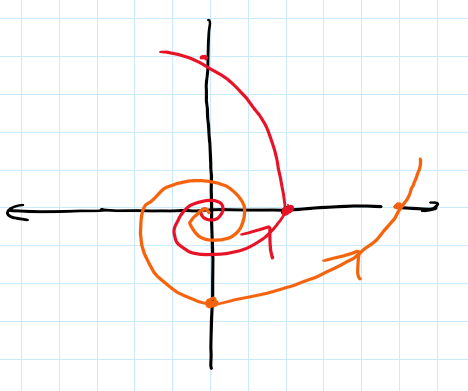
\includegraphics[height=1.5in]{Images/phaseportrait_1_n2_2_1_sketch.png}}\hfill\hfill
%}

\begin{exercise}%
    Solve $x_1' = x_2$, $x_2' = -x_1$ using the eigenvalue method.
\end{exercise}
%\exsol{%
%$\vec{x} =
%C_1 \left[ \begin{smallmatrix}
%\cos(t) \\ -\sin(t)
%\end{smallmatrix}\right]
%+
%C_2 \left[ \begin{smallmatrix}
%\sin(t) \\ \cos(t)
%\end{smallmatrix}\right]$ \hfill\raisebox{-0.5\height}{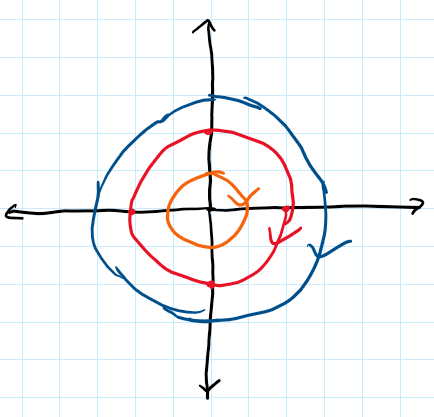
\includegraphics[height=1.5in]{Images/phaseportrait_0_1_n1_0_sketch.png}}\hfill\hfill
%}

\begin{exercise}
    A $2\times 2$ matrix $A$ has complex eigenvector $\displaystyle \vec{v}=\begin{bmatrix} 1\\ i \end{bmatrix}$ corresponding to eigenvalue $\lambda=-1+3i$. %4.5
    \begin{tasks}
        \task Use Euler's Formula to find the (real-valued) general solution to the system $\vec{x}'=A\vec{x}$.
        \task Sketch the phase portrait of this system.
    \end{tasks}
\end{exercise}
%\comboSol
%{%
%$\vec{x}(t) = C_1e^{-t}\left[\begin{smallmatrix} \cos(3t)\\ -\sin(3t) \end{smallmatrix}\right] + C)2e^{-t}\left[\begin{smallmatrix} \sin(3t)\\ \cos(3t) \end{smallmatrix}\right]$  \hfill\raisebox{-0.5\height}{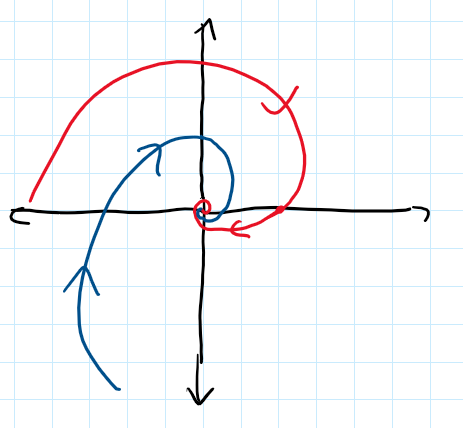
\includegraphics[height=1.5in]{Images/phaseportrait_sketch_fromevec_complex.png}}\hfill\hfill
%}

\begin{exercise}%
    \begin{tasks}
        \task Compute eigenvalues and eigenvectors of
            $A=\left[ 
                \begin{smallmatrix}
                    1 & 1 \\
                    -1 & 0 
                \end{smallmatrix}
            \right]$.
        \task Solve the system $\vec{x}\,' = A\vec{x}$.
        \task Sketch the phase portrait for this system
    \end{tasks}
\end{exercise}
%\exsol{%
%a)
%Eigenvalues: $\frac{1+\sqrt{3}i}{2},
%\frac{1-\sqrt{3}i}{2}$,
%\quad
%Eigenvectors:
%$\left[ \begin{smallmatrix}
%-2 \\ 1-\sqrt{3}i
%\end{smallmatrix}\right]$,
%$\left[ \begin{smallmatrix}
%-2 \\ 1+\sqrt{3}i
%\end{smallmatrix}\right]$
%\\
%b)
%$\vec{x} = C_1
%e^{t/2}
%\left[ \begin{smallmatrix}
%-2\cos\bigl(\frac{\sqrt{3}t}{2}\bigr)
%\\
%\cos\bigl(\frac{\sqrt{3}t}{2}\bigr) + \sqrt{3}\sin\bigl(\frac{\sqrt{3}t}{2}\bigr)
%\end{smallmatrix}\right]
%+
%C_2
%e^{t/2}
%\left[ \begin{smallmatrix}
%- 2\sin\bigl(\frac{\sqrt{3}t}{2}\bigr)
%\\
%\sin\bigl(\frac{\sqrt{3}t}{2}\bigr) -\sqrt{3}\cos\bigl(\frac{\sqrt{3}t}{2}\bigr)
%\end{smallmatrix}\right]$ \quad c)~ \hfill\raisebox{-0.5\height}{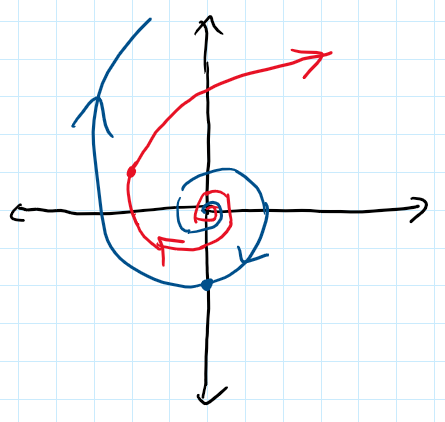
\includegraphics[height=1.5in]{Images/phaseportrait_1_1_n1_0_sketch.png}}\hfill\hfill
%}

\begin{exercise}
    Consider the system
    \begin{equation*}
        \begin{bmatrix} 
            x' \\ 
            y' 
        \end{bmatrix} 
        = 
        \begin{bmatrix} 
            1& -2 \\ 
            5 & -1 
        \end{bmatrix} 
        \begin{bmatrix} 
            x \\ 
            y 
        \end{bmatrix}.
    \end{equation*} %4.5
    \begin{tasks}
        \task Find the general solution.
        \task Sketch the phase portrait for this system.
        \task Solve the IVP with initial conditions $x(0)=1, y(0)=0$, and determine the maximum $x$-coordinate on this trajectory.
    \end{tasks}
\end{exercise}
%\comboSol
%{%
%a)~$C_1\left[\begin{smallmatrix} 2\cos(3t) \\ \cos(3t) + 3\sin(3t) \end{smallmatrix}\right] + C_2 \left[\begin{smallmatrix} 2\sin(3t) \\ \sin(3t) - 3\cos(3t) \end{smallmatrix}\right]$ \quad b)~ \hfill\raisebox{-0.5\height}{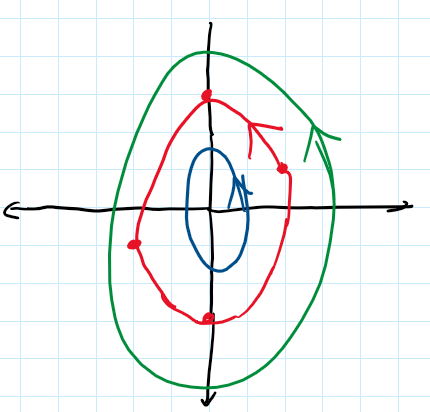
\includegraphics[height=1.5in]{Images/phaseportrait_1_n2_5_n1_sketch.png}}\hfill\hfill c)~$x = \frac{\sqrt{10}}{3}$
%}

\begin{exercise}%%
    Find the general solution of the system
    \begin{equation*}
        {\vec{x}}' = 
        \begin{bmatrix} 
            4 & 1 \\ 
            -5 & 2 
        \end{bmatrix} \vec{x}
    \end{equation*}
    and sketch the phase portrait for this system.
\end{exercise}
%\comboSol
%{%
%$\vec{x}(t) = C_1e^{3t} \left[\begin{smallmatrix} -\cos(2t) \\ \cos(2t) + 2\sin(2t) \end{smallmatrix}\right] + C_2e^{3t}\left[\begin{smallmatrix} -\sin(2t) \\ \sin(2t) - 2 \cos(2t) \end{smallmatrix}\right]$ \hfill\raisebox{-0.5\height}{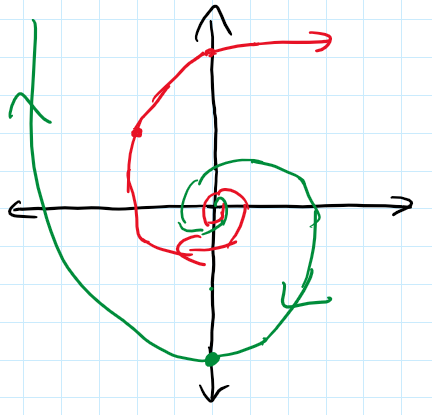
\includegraphics[height=1.5in]{Images/phaseportrait_4_1_n5_2_sketch.png}}\hfill\hfill
%}


\begin{exercise}%%
    Find the general solution of the system
    \begin{equation*}
        {\vec{x}}' = 
        \begin{bmatrix} 
            1 & 4 \\ 
            -2 & -3 
        \end{bmatrix} \vec{x}
    \end{equation*}
    and sketch the phase portrait for this system.
\end{exercise}
%\comboSol
%{%
%$\vec{x}(t) = C_1e^{-t}\left[\begin{smallmatrix} \cos(2t) - \sin(2t) \\ -\cos(2t) \end{smallmatrix}\right] + C_2e^{-t}\left[\begin{smallmatrix} \sin(2t) + \cos(2t) \\ -\sin(2t) \end{smallmatrix}\right]$ \hfill\raisebox{-0.5\height}{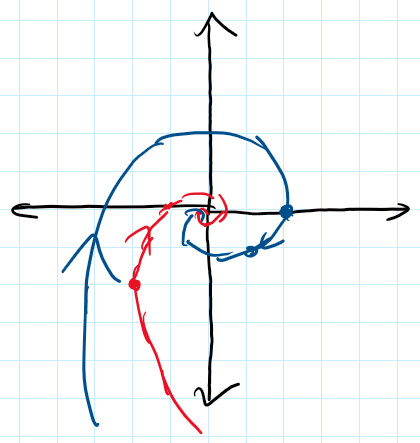
\includegraphics[height=1.5in]{Images/phaseportrait_1_4_n2_n3_sketch.png}}\hfill\hfill
%}

\begin{exercise}%%
    Find the general solution of the system
    \begin{equation*}
        {\vec{x}}' = 
        \begin{bmatrix} 
            2 & 0 & 3 \\ 
            -6 & 2 & -9 \\ 
            -3 & 0 & 2 
        \end{bmatrix} \vec{x}.
    \end{equation*}
\end{exercise}
%\comboSol
%{%
%$\vec{x}(t) = C_1\left[\begin{smallmatrix} 0 \\ 1 \\ 0 \end{smallmatrix}\right]e^{2t} + C_2e^{2t}\left[\begin{smallmatrix} \cos(3t) \\ -2\cos(3t) - 2\sin(3t)\\ -\sin(3t) \end{smallmatrix}\right] + C_3e^{2t}\left[\begin{smallmatrix} \sin(3t) \\ 2\cos(3t) - 3\sin(3t) \\ \cos(3t) \end{smallmatrix}\right]$
%}

\begin{exercise}%%
    Find the general solution of the system
    \begin{equation*}
        {\vec{x}}' = 
        \begin{bmatrix} 
            -10 & -4 & 0 \\ 
            14 & 4 & 1 \\ 
            12 & 6 & -2 
        \end{bmatrix} \vec{x}.
    \end{equation*}
\end{exercise}
%\comboSol
%{%
%$\vec{x}(t) = C_1\left[\begin{smallmatrix} -1 \\ 2 \\ 2 \end{smallmatrix}\right]e^{-2t} + C_2e^{-3t} \left[\begin{smallmatrix} -4\cos(t) \\ 7\cos(t) - \sin(t) \\ 6\cos(t)  \end{smallmatrix}\right] + C_2e^{-3t}\left[\begin{smallmatrix} -4\sin(t) \\ 7\sin(t) + \cos(t) \\ 6\sin(t) \end{smallmatrix}\right]$
%}

\begin{exercise}
    Solve the initial value problem
    \[ 
        {\vec{x}}' = 
        \begin{bmatrix} 
            3 & -1 \\ 
            4 & 3 
        \end{bmatrix} 
        \vec{x} \qquad \vec{x}(0) = 
        \begin{bmatrix} 
            2 \\ 
            -1 
        \end{bmatrix}. 
    \]
\end{exercise}
%\comboSol
%{%
%$\vec{x}(t) = e^{3t} \left[\begin{smallmatrix}2\cos(2t) + \frac{1}{2}\sin(2t) \\ -\cos(2t) + 4\sin(2t) \end{smallmatrix}\right]$
%}


\begin{exercise}
    Solve the initial value problem
    \[ 
        {\vec{x}}' = 
        \begin{bmatrix} 
            -8 & -8 \\ 
            5 & 4 
        \end{bmatrix} 
        \vec{x} \qquad \vec{x}(0) = 
        \begin{bmatrix} 
            1 \\ 
            1 
        \end{bmatrix}. 
    \]
\end{exercise}
%\comboSol
%{%
%$\vec{x}(t) = e^{-2t}\left[\begin{smallmatrix} \cos(2t) - 7\sin(2t)\\ \cos(2t) + \frac{11}{2}\sin(2t) \end{smallmatrix}\right]$
%}

\begin{exercise}
    Solve the initial value problem
    \[ 
        {\vec{x}}' = 
        \begin{bmatrix}
            -1 & 2 & -8 \\ 
            0 & 1 & -4 \\ 
            0 & 2 & -3 
        \end{bmatrix} 
        \vec{x} \qquad \vec{x}(0) = 
        \begin{bmatrix} 
            2 \\ 
            1 \\ 
            -3 
        \end{bmatrix}. 
    \]
\end{exercise}
%\comboSol
%{%
%$\vec{x}(t) = e^{-t}\left[\begin{smallmatrix} -7 + 5\cos(2t) + 13\sin(2t) \\ \cos(2t) + 7\sin(2t) \\ -3\cos(2t) + 4\sin(2t) \end{smallmatrix}\right]$
%}

\end{document}